\chapter{System Details}


The electroplating system is an unstable system that relies on multiple parameters being within their respective optimal ranges to achieve a desired mode. 
Several tips can help reduce noise and stabilize the system, such as avoiding the use of an oscilloscope with the charger to avoid power line noise. 
Mechanical noise in the pumping machine can be minimized by using a syringe pump tilted with a bubble inside. 
External electrical noise can be picked up by antennas or connections in the circuit. 
To stabilize internal humidity, turn on the gas pipeline with air into the chamber.

The picture in figure \ref{fig:setup_pic} shows the setup used in all this project. Figure \ref{fig:nozzleElectr} shows the nozzle and plate with the charged liquid being electrosprayed in cone jet mode.

\begin{figure}[H]
  \centering
  \resizebox{150mm}{!}{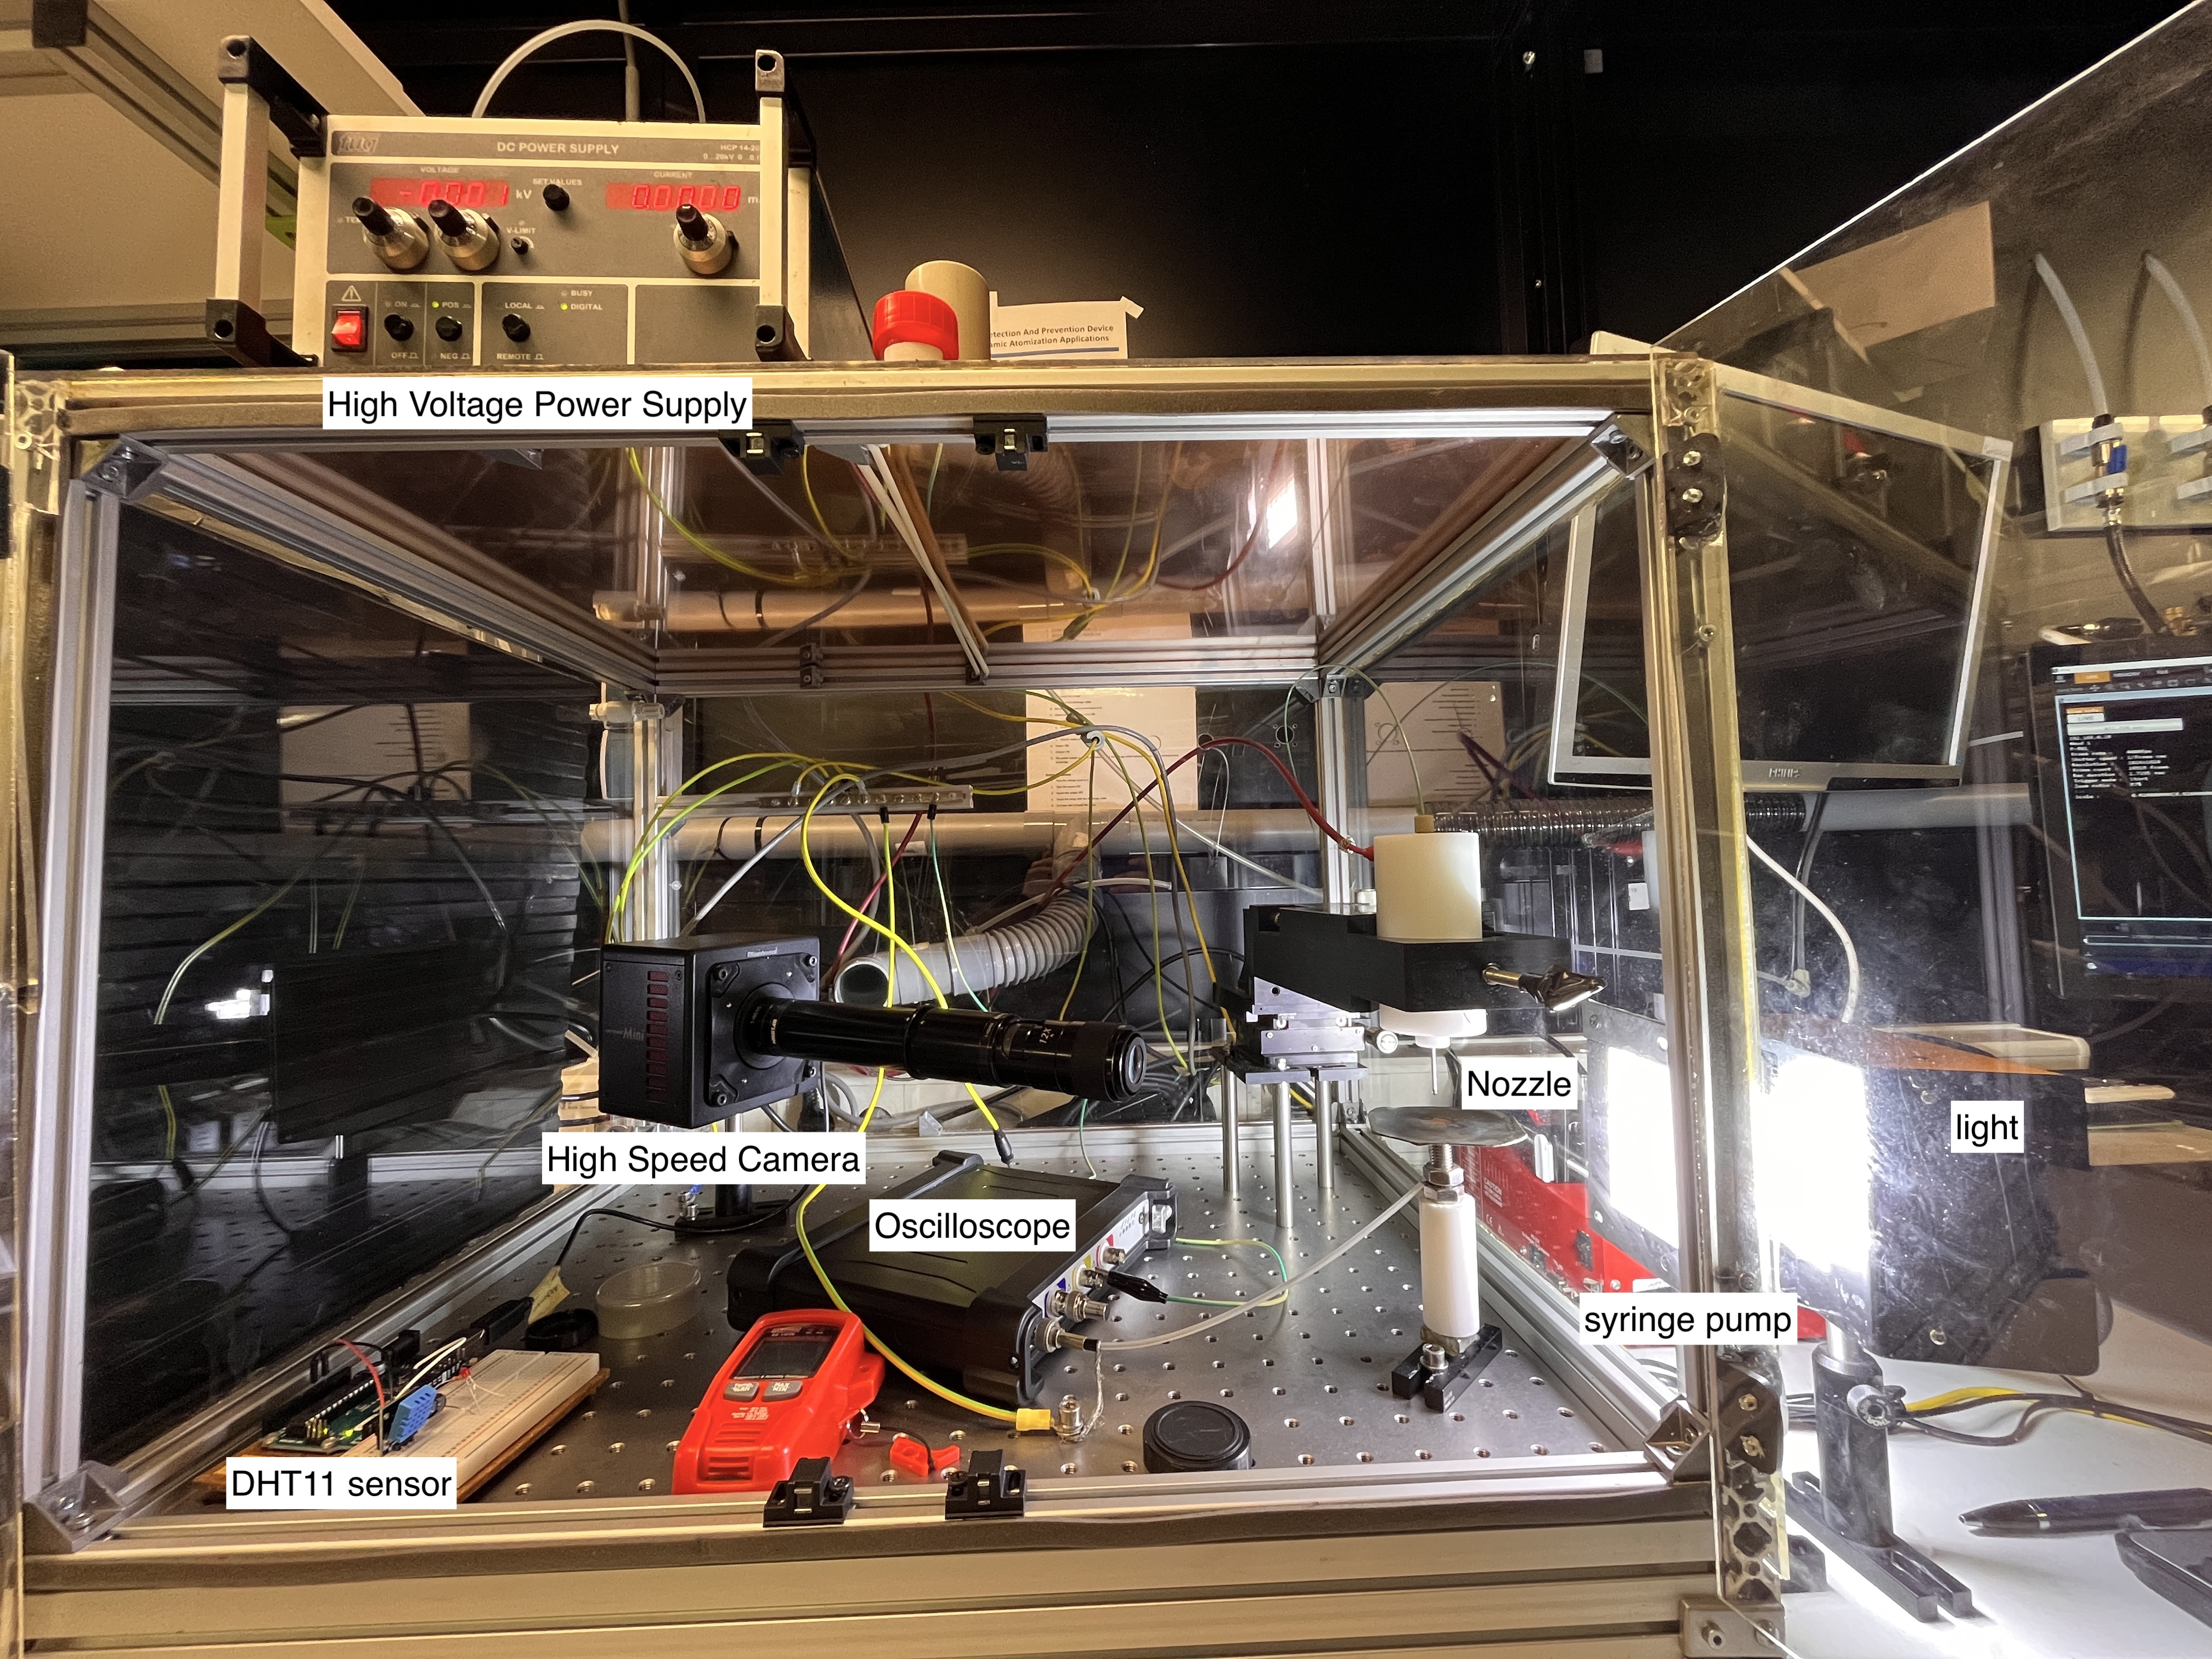
\includegraphics{Figuras/setup_pic.jpg}}
  \caption{EHDA automation system setup used for experiments.}
  \label{fig:setup_pic}
\end{figure}

\begin{figure}[H]
    \centering
    \resizebox{80mm}{!}{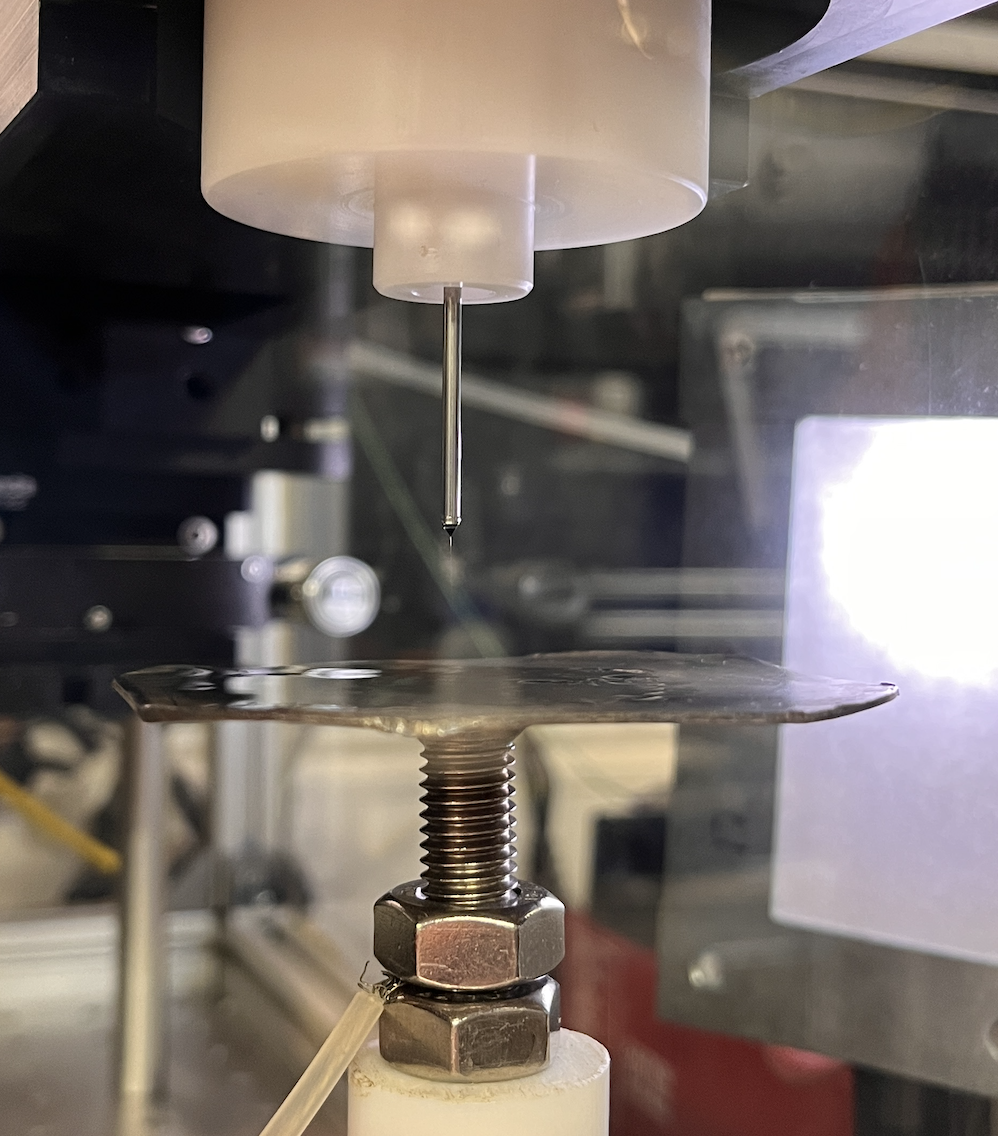
\includegraphics{Figuras/naked_eyes.png}}
    \label{fig:nozzleElectr}
    \caption{EHDA picture of the electrified syringe.}
\end{figure}


\section{Setup Validation}
\label{sec:setup_validation}


It is recommended to do initial tests in order to verify the setup assembly and the automation routine integration. 
This is an important step to understand in practice how electrospray works.
Factors like geometry, polarity, material properties and occurring discharges are reflected in the system current.
Also, liquid properties such as surface tension, dielectric constant, viscosity, density, electrical conductivity and vacuum permittivity. 
And also physical variables such as flow rate, system impedance, system temperature, system humidity, nozzle to plate distance, nozzle dimensions and applied voltage.


\section{Oscilloscope Impedance}
\label{sec:osc_impedance}

The current being measured by the Oscilloscope use its internal impedance. 
The \emph{TiePie} oscilloscope model has two impedance options, 1Mohm or 2Mohms. 
Selecting one or other will multiply or divide your current measurement by 2. 
By default, it is being used 2Mohm differential input, however it was noticed that using the 1Mohm resistance might reduce noise. 
A proposal is to configure the 1Mohm resistance in the \emph{configuration\_tiepie.py} file and evaluate its performance.